Given that the substitution cipher is used, I do frequency analysis to find
the most frequent figure (letter) in this case. In order to count the frequency,
I need firstly encode each figure into a bit string fed into the Python script.
An example is illustrated in \autoref{fig:encode_bits}. It is found that the
most frequent encoded figure is \emph{`110000'}, 34 occurences, which should be
replaced by \emph{`E'}. Then, I tried to find the most frequent 3-grams. I found that
\emph{(`000110', `001010', `110000')} with 6 occurences is the most frequent 3-grams,
which should be substituted by \emph{`THE'}. From these two findings, I can detect
the following replacement: \emph{(`000110':`T'), (`001010':`H'), (`110000':`E')}.

\begin{figure}
    \centering
    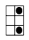
\includegraphics[width=\textwidth,height=\textheight,keepaspectratio]
    {figures/encoded_figure.png}
    \caption{A figure is encoded into '010001' bit string.}\label{fig:encode_bits}
\end{figure}